\documentclass{article}
\usepackage{graphicx}

\begin{document}

\begin{center}
\begin{large}
\textbf{Wednesday, January 22, 2014}
\end{large}
\end{center}

\section{My First Pictures in \LaTeX{}}

We've saved a picture as a .jpg or .png (only kind that will work in a pdf from
\LaTeX{}).

You need to add 
\begin{verbatim}
\usepackage{graphicx}
\end{verbatim}
to our preface

To add the picture we type
\begin{verbatim}
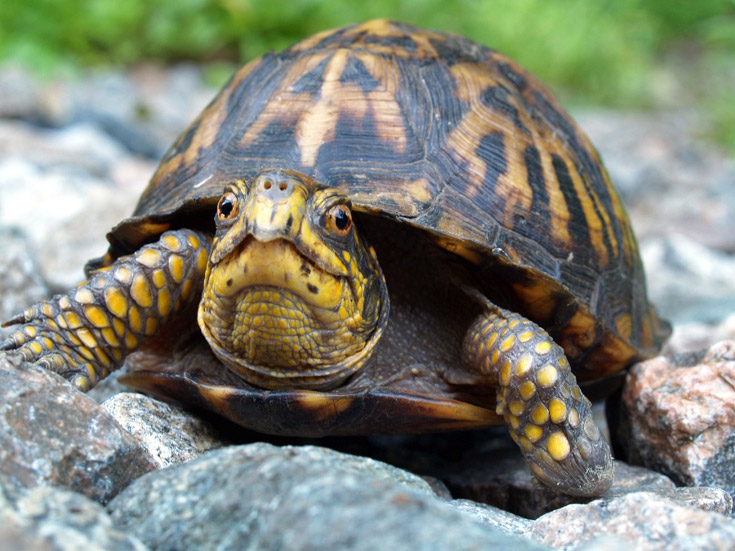
\includegraphics[scale=.5]{eastern-box-turtle.jpg}
\end{verbatim}
Now we use it in our document
\begin{center}
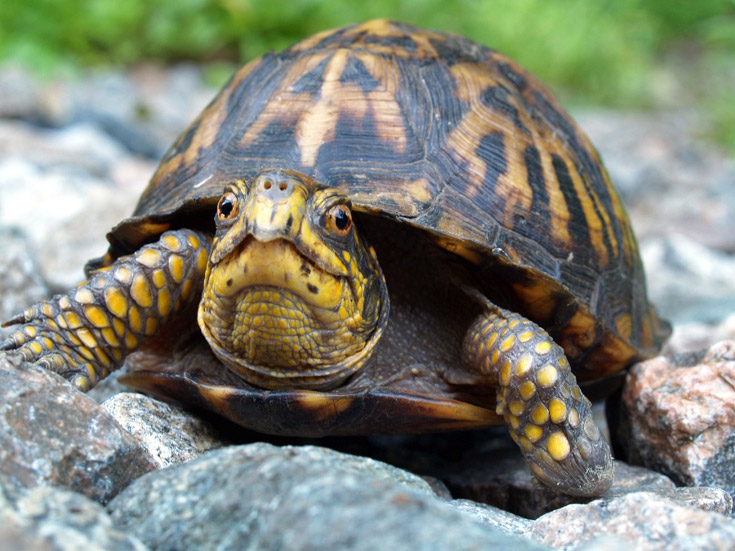
\includegraphics[scale=.5]{eastern-box-turtle.jpg}
\end{center}

To actually create a figure with a caption:

\begin{figure}[h!]
\includegraphics[width=3in,angle=45][scale=.25]{eastern-box-turtle.jpg}
\caption{This is my first formal figure}
\end{figure}

\end{document}
